\documentclass[]{book}
\usepackage{lmodern}
\usepackage{amssymb,amsmath}
\usepackage{ifxetex,ifluatex}
\usepackage{fixltx2e} % provides \textsubscript
\ifnum 0\ifxetex 1\fi\ifluatex 1\fi=0 % if pdftex
  \usepackage[T1]{fontenc}
  \usepackage[utf8]{inputenc}
\else % if luatex or xelatex
  \ifxetex
    \usepackage{mathspec}
  \else
    \usepackage{fontspec}
  \fi
  \defaultfontfeatures{Ligatures=TeX,Scale=MatchLowercase}
\fi
% use upquote if available, for straight quotes in verbatim environments
\IfFileExists{upquote.sty}{\usepackage{upquote}}{}
% use microtype if available
\IfFileExists{microtype.sty}{%
\usepackage{microtype}
\UseMicrotypeSet[protrusion]{basicmath} % disable protrusion for tt fonts
}{}
\usepackage[margin=1in]{geometry}
\usepackage{hyperref}
\hypersetup{unicode=true,
            pdftitle={Manual of preparation and transformation of open data},
            pdfauthor={Juan Ramírez},
            pdfborder={0 0 0},
            breaklinks=true}
\urlstyle{same}  % don't use monospace font for urls
\usepackage{natbib}
\bibliographystyle{apalike}
\usepackage{longtable,booktabs}
\usepackage{graphicx,grffile}
\makeatletter
\def\maxwidth{\ifdim\Gin@nat@width>\linewidth\linewidth\else\Gin@nat@width\fi}
\def\maxheight{\ifdim\Gin@nat@height>\textheight\textheight\else\Gin@nat@height\fi}
\makeatother
% Scale images if necessary, so that they will not overflow the page
% margins by default, and it is still possible to overwrite the defaults
% using explicit options in \includegraphics[width, height, ...]{}
\setkeys{Gin}{width=\maxwidth,height=\maxheight,keepaspectratio}
\IfFileExists{parskip.sty}{%
\usepackage{parskip}
}{% else
\setlength{\parindent}{0pt}
\setlength{\parskip}{6pt plus 2pt minus 1pt}
}
\setlength{\emergencystretch}{3em}  % prevent overfull lines
\providecommand{\tightlist}{%
  \setlength{\itemsep}{0pt}\setlength{\parskip}{0pt}}
\setcounter{secnumdepth}{5}
% Redefines (sub)paragraphs to behave more like sections
\ifx\paragraph\undefined\else
\let\oldparagraph\paragraph
\renewcommand{\paragraph}[1]{\oldparagraph{#1}\mbox{}}
\fi
\ifx\subparagraph\undefined\else
\let\oldsubparagraph\subparagraph
\renewcommand{\subparagraph}[1]{\oldsubparagraph{#1}\mbox{}}
\fi

%%% Use protect on footnotes to avoid problems with footnotes in titles
\let\rmarkdownfootnote\footnote%
\def\footnote{\protect\rmarkdownfootnote}

%%% Change title format to be more compact
\usepackage{titling}

% Create subtitle command for use in maketitle
\newcommand{\subtitle}[1]{
  \posttitle{
    \begin{center}\large#1\end{center}
    }
}

\setlength{\droptitle}{-2em}
  \title{Manual of preparation and transformation of open data}
  \pretitle{\vspace{\droptitle}\centering\huge}
  \posttitle{\par}
  \author{Juan Ramírez}
  \preauthor{\centering\large\emph}
  \postauthor{\par}
  \predate{\centering\large\emph}
  \postdate{\par}
  \date{2017-05-03}

\usepackage{booktabs}
\usepackage{amsthm}
\makeatletter
\def\thm@space@setup{%
  \thm@preskip=8pt plus 2pt minus 4pt
  \thm@postskip=\thm@preskip
}
\makeatother

\begin{document}
\maketitle

{
\setcounter{tocdepth}{1}
\tableofcontents
}
\chapter{Overview}\label{overview}

This manual describes through a methodology the activities of
extraction, cleaning and integration of data bases prior to the
processing and analysis phase. In addition to this manual and using a
programming environment, automated scripts are developed for cleaning,
integrating and transforming data.

\chapter{The Methodology}\label{methodology}

\section{Introduction}\label{introduction}

In this chapter we present the methodology that we used to work with the
data. We will explain each step individually and as part of the many
subprocesses that are required to understand the databases present in
datos.gob.mx.

\section{General Model of the
Methodology}\label{general-model-of-the-methodology}

The purpose of this methodology is to turn the raw databases found in
the portal into understanding, insight and knowledge. To accomplish
this, there is a need for using a computing system, for we will be using
the statistical software R, which is free and open source.

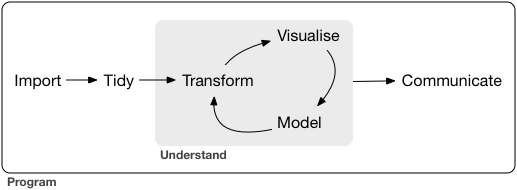
\includegraphics{diagrams/data-science.png}

\subsection{Individual Steps of the
Methodology}\label{individual-steps-of-the-methodology}

\subsubsection{Import}\label{import}

First you must import your data into R. This typically means that you
take data stored in a file, database, or web API, and load it into a
data frame in R. In this step is where you usually deal with encoding,
language, and formats issues.

\subsubsection{Tidy}\label{tidy}

Once you've imported your data, it is a good idea to tidy it. Tidying
your data means storing it in a consistent form that matches the
semantics of the dataset with the way it is stored. In brief, when your
data is tidy, each column is a variable, and each row is an observation.
Tidy data is important because the consistent structure lets you focus
your struggle on questions about the data, not fighting to get the data
into the right form for different functions.

\subsubsection{Transformation}\label{transformation}

Once you have tidy data, a common first step is to transform it.
Transformation includes narrowing in on observations of interest (like
all people in one city, or all data from the last year), creating new
variables that are functions of existing variables (like computing
velocity from speed and time), and calculating a set of summary
statistics (like counts or means). Together, tidying and transforming
are called wrangling, because getting your data in a form that's natural
to work with often feels like a fight!

\subsubsection{Visualisation and
Modelling}\label{visualisation-and-modelling}

Once you have tidy data with the variables you need, there are two main
engines of knowledge generation: visualisation and modelling. These have
complementary strengths and weaknesses so any real analysis will iterate
between them many times.

Visualisation is a fundamentally human activity. A good visualisation
will show you things that you did not expect, or raise new questions
about the data. A good visualisation might also hint that you're asking
the wrong question, or you need to collect different data.
Visualisations can surprise you, but don't scale particularly well
because they require a human to interpret them.

Models are complementary tools to visualisation. Once you have made your
questions sufficiently precise, you can use a model to answer them.
Models are a fundamentally mathematical or computational tool, so they
generally scale well. Even when they don't, it's usually cheaper to buy
more computers than it is to buy more brains! But every model makes
assumptions, and by its very nature a model cannot question its own
assumptions. That means a model cannot fundamentally surprise you.

\subsubsection{Communication}\label{communication}

The last step of the methodology is communication, an absolutely
critical part of any data analysis project. It doesn't matter how well
your models and visualisation have led you to understand the data unless
you can also communicate your results to others.

\subsubsection{Programming}\label{programming}

Surrounding all these tools is programming. Programming is a
cross-cutting tool that you use in every part of the project. You don't
need to be an expert programmer to be a data scientist, but learning
more about programming pays off because becoming a better programmer
allows you to automate common tasks, and solve new problems with greater
ease.

\subsection{Parts of the process}\label{parts-of-the-process}

To accomplish this methodology, we will divide the whole process into
several pieces that we explain next.

\subsubsection{Wrangling the Data}\label{wrangling-the-data}

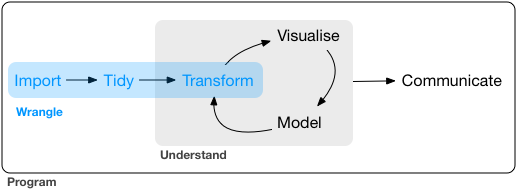
\includegraphics{diagrams/data-science-wrangle.png}

The objective of the wrangling phase of the method is to resolve all the
informatical issues around the database. As mentioned before, the final
goal to achieve is to tidy all the databases involved. For this task, R
(and more specifically, the tidyverse package) supplies mostly of the
tools you will need to get your data in a consistent form.

\subsubsection{Exploring the data}\label{exploring-the-data}

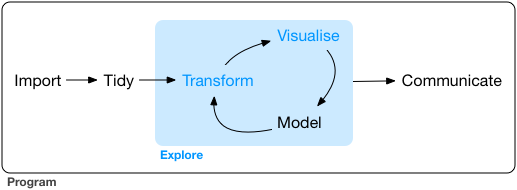
\includegraphics{diagrams/data-science-explore.png}

When the data has already been tidied, the first step in the analysis is
exploring the data. This means that you want to find as many
relationships and irregularities as possible. For this, the main tools
are visualisation and transformation which are generally applied in the
following way:

\begin{enumerate}
\def\labelenumi{\arabic{enumi}.}
\tightlist
\item
  You generate questions about your data.
\item
  Search for answers by visualising, transforming, and modelling your
  data.
\item
  Use what you learn to refine your questions and/or generate new
  questions.
\end{enumerate}

\subsubsection{Communicating}\label{communicating}

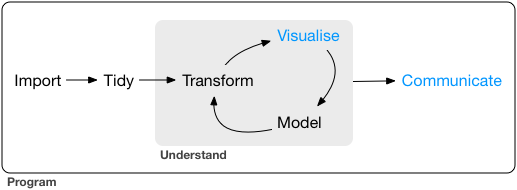
\includegraphics{diagrams/data-science-communicate.png}

The final step in the methodology is to wrap up all the wrangling,
exploration, and modelling in a single report. For this task is very
useful to recycle all the plots that you have already used to explore
the data. As a technological tool, the R environment (in a very similar
manner to the Python environment) allows us to put the plots, text and R
code in a single document called Analysis Notebook.

\chapter{The Extraction Phase}\label{the-extraction-phase}

\section{Introduction}\label{introduction-1}

Even while the obtaining of the data is not part of the analysis
methodology, we have to point out that it is no trivial matter to obtain
data to begin working with. It is important to note also that this part
of the process depends completely upon the structure and contents of the
portal. There is no way to design a general method for obtaining data
because each database is constructed and obtained in its own way. Even
so, we will try to explain what have we done in this particular
case(mexican open government data stored in datos.gob.mx) in order to
clear the path for future investigations.

\section{The CKAN system and its API}\label{the-ckan-system-and-its-api}

The data portal datos.gob.mx is built upon the design and
functionalities of the CKAN system. To better explain how to use the
portal, we first present a brief overview of CKAN, the definition of API
and how it is related to our problem.

The first key concept is CKAN. Quoting from the CKAN website, ``CKAN is
a powerful data management system that makes data accessible -- by
providing tools to streamline publishing, sharing, finding and using
data. CKAN is aimed at data publishers (national and regional
governments, companies and organizations) wanting to make their data
open and available''.

The second key topic is the concept of API. An Application Programming
Interface (API) is a set of subroutine definitions, protocols, and tools
for building application software. In general terms, it is a set of
clearly defined methods of communication between various software
components.

Finally, we have to link these key ideas together:

The portal datos.gob.mx is an implementation of the CKAN system which is
a platform to publish open data and make it accesible. CKAN has many
tools in order to accomplish the accesibility of the data: it has a tag
system, a query system, and a way of organizing the databases that makes
it very easy to find the desired data. To make it possible for a program
to access the site, CKAN has a set of functions (called API) which
allows a program to make use of the all the functionality that the site
has.

\section{Keywords}\label{keywords}

The first step to obtain data is to try to guess the tags that are
associated to the database. This a heuristic task for which we present a
useful resource: list all the tags available in the site. This is most
useful when you already know how to use the site (for which we mean
knowing how to use the CKAN API), but you can use this tip querying on
the search bar of the site.

\section{Identifying the source of the
data}\label{identifying-the-source-of-the-data}

After identifying

\section{Discriminate the irrelevant
entries}\label{discriminate-the-irrelevant-entries}

\section{Download}\label{download}

\section{Checking the data}\label{checking-the-data}

\chapter{Prerequisites}\label{prerequisites}

\section{Introduction}\label{introduction-2}

In this chapter we will present the preparation steps needed in order to
be able to analyse a database of datos.gob.mx. The most important notion
of this chapter is the concept of tidy data, which is a consistent form
of arranging the data in a dataset that enables us to work more
eficiently and stay focused analysing the data.

\section{Software}\label{software}

\subsection{What is R?}\label{what-is-r}

The software we chose to analyse the data contained in datos.gob.mx is
called R. This is a programming language and ecosystem made for
statistical analysis that is free and open source. We chose R because it
is free software, which is a way of fulfilling the preconditions needed
for anyone to make use of the free and open databases in datos.gob.mx.

\subsection{R}\label{r}

The best source to install R is CRAN, the Complete R Archive Network
\url{https://cran.r-project.org/} . In this website there are many
guides with the instructions needed to install R in a variety of
operating systems, such as Windows, Mac and Linux. The basic tools that
we used are already included in the Debian package named ``r-base''.

\subsection{RStudio}\label{rstudio}

When facing a programming language, it is often useful to have a IDE
(short for Integrated Development Environment). An ideal IDE makes it
more eficient to write programs because it saves the user a lot of
typing and also may have many useful functions such as browsing files,
show dependencies between the programs, highlighting the code (which
makes easier to spot the structure of the program), variable browser,
etc. The IDE we chose for using with R is called RStudio, which is made
for statistical analysis and also is free and open source, like R. The
ecosystem of R and RStudio makes it possible to analyse the data in many
different ways, printing plots and making complete reports of the
analysis among many others. All these functionalities make it ideal to
analyse the datasets in the portal. RStudio can be downloaded in
\url{https://www.rstudio.com/}

\subsection{The tidyverse}\label{the-tidyverse}

The R ecosystem is very extensible and customizable via something called
\textbf{packages}. An R package is a collection of functions, data, and
documentation that extends the capabilities of base R. The tidyverse is
a wrapper around many packages that work consistently with data and have
as a whole almost any tool needed in order to analyse a database. The
tidyverse includes packages to do almost all the steps in the
methodology: making plots about a dataset, transform the variables of a
dataset, importing a dataset and resolving its encoding issues, fitting
a mathematical model to a variable, among many others. As all these
packages are linked together, the tidyverse implements a set of
consistent names, functions and tools to make it easier to have all its
parts work together on a single dataset.

\section{Tidy data}\label{tidy-data}

\subsection{\texorpdfstring{Why would we ``tidy'' the
data?}{Why would we tidy the data?}}\label{why-would-we-tidy-the-data}

The final prerequisite to begin working with the databases in the portal
is to understand what means that a dataset is tidy. The tidy data is a
way to resolve all the differences between the many formats, structures,
and encodings that databases can have. It also allows us to work the
database with the tidyverse, saving us the time to put the database in a
different form for plotting, transforming or modelling. It also makes it
easier for R to work with the database because the inherent variable
that R uses is a \textbf{vector}, (which is a ordered tuple of data of
the same kind) and every column in a tidy dataset is a vector.

\subsection{Variables}\label{variables}

The basis of the concept of tidy data is the idea of a measurable
feature of something. For example, the speed of a car, the height of a
person and the date of an event are all measurable features of the
respective objects. The way in which this concept leads to the tidying
of a dataset is that because a variable is a measurable thing, maybe it
is a number or date o category, so we can make the computer understand
it. As R uses vectors as its basic blocks, we want variables to be
encoded in vectors. This is the reason why we are going to put all the
variables in columns, which makes the first step in the tidying of a
dataset.

\subsection{Observations}\label{observations}

As variables make the measurable aspects of something, we can speak of
the ``instant'' in which we measured the data of the something. For
example, if we are studying diseases in country, we can talk about the
number of diseased people, the country and dead people, all of which are
linked together by the variable year, which is the moment in which all
the other variables happened in the way we are trying to study. Putting
together all the values of the measured variables, we can think of a
concrete situation, so it makes sense to put all this data together in a
way. This is the reason why we are going to put the observations as the
rows of the dataset, which is the final step in the tidying of a
dataset.

\subsection{Definition and Example}\label{definition-and-example}

Having all these ideas at hand, we finally define tidy data:

\begin{itemize}
\item
  All the variables in the dataset have its own column.
\item
  All the observations of the variables have its own row.
\end{itemize}

In a picture, this is what we call tidy data:

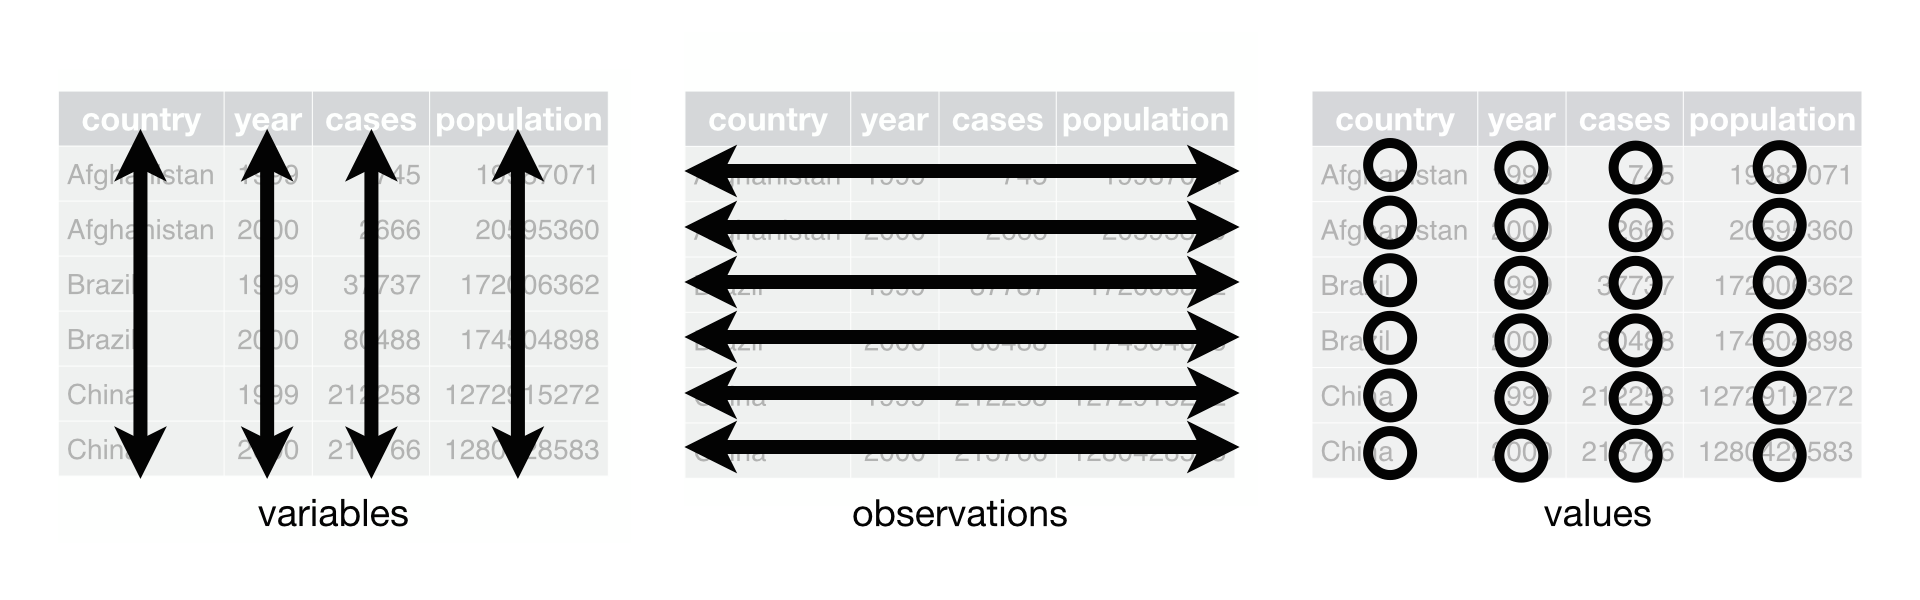
\includegraphics{images/tidy-1.png}

\chapter{Applications}\label{applications}

Some \emph{significant} applications are demonstrated in this chapter.

\section{Example one}\label{example-one}

\section{Example two}\label{example-two}

\chapter{Final Words}\label{final-words}

We have finished a nice book.

\bibliography{packages.bib,book.bib}


\end{document}
